\documentclass{scrartcl}

\usepackage{german}
\usepackage[utf8]{inputenc}  %Umlaute
\usepackage[T1]{fontenc}     %Umlauttrennung
\usepackage{lmodern}         %modernes Schriftbild
\usepackage{amsmath}         %math Umgebungen
\usepackage{graphicx}
\usepackage{hyperref}        %URLs
\usepackage{gensymb}         %Gradzeichen
\usepackage{float}           %Positionierung von Tabellen und Abb

\title{Physikpraktikum für Naturwissenschaftler \\ Versuch: Beugung}
\author{Felix Burr, Johannes Spindler (Gruppe 13)}
\date{Durchgeführt am 06. Dezember 2018}


\begin{document}
\begin{titlepage}
  \begin{center}
    \vspace*{1cm}
    \LARGE
    Physikpraktikum für Naturwissenschaftler \\
    \vspace*{1cm}
    \Huge
    \textbf{Versuch: Beugung} \\
    \vspace*{0.3cm}
    \Large
    Durchgeführt am 06. Dezember 2018 \\
    Betreuer: Devin Assenheimer \\
    \vspace*{2.5cm}
    Gruppe 13 \\
    Felix Burr: felix.burr@uni-ulm.de \\
    Johannes Spindler: johannes.spindler@uni-ulm.de \\
    \vfill 
  \end{center}
  Wir bestätigen hiermit, das Protokoll selbstständig erarbeitet zu haben und in genauer Kenntnis über dessen Inhalt zu sein. \\
  \vspace*{0.8cm}
  \\
  Felix Burr
  \hfill
  Johannes Spindler
\end{titlepage}
\pagebreak
\tableofcontents


\pagebreak

\section{Einleitung}
Unter Beugung wird die Ausbreitung von Wellen in den Schattenbereich hinter Objekten verstanden. Da Beugung für Wellen auftritt, aber nicht für Teilchen, ist die Beugung von Licht ein Indiz für dessen Wellencharakter. Mithilfe des Strahlenmodells des Lichts ist die Beugung nicht erklärbar und die Geometrische Optik mit ihrem Strahlenmodell ist auch nur eine Annäherung an die Realität, da sie nutzt, dass die Beugung des Lichts vernachlässigbar ist, wenn Öffnungen und Hindernisse sehr viel größer sind als die Wellenlänge des Lichts. Das Phänomen der Beugung ist sehr nützlich bei der Untersuchung von Objekten. So kann zum Beispiel die Spaltbreite eines Gitters, die Gitterkonstante, berechnet werden (siehe Abschnitt 2) oder ein chemisches Element durch die Spektralanalyse bestimmt werden (siehe Abschnitt 4).

\section{Strukturaufklärung (Bestimmung einer Gitterkonstanten)}
\subsection{Versuchsdurchführung}
Das zu untersuchende Gitter mit Gitterkonstante $g$ wird mit einem HeNe-Laser der Wellenlänge $\lambda = 632,8nm$ beleuchtet. Die Wand dient als Schirm, weshalb der Laser so positioniert sein soll, dass der Strahl senkrecht zur Wand verläuft. Es erscheinen Beugungsmaxima auf der Wand. Abbildung \ref{fig:Gitter} zeigt diese Versuchsanordnung.
\begin{figure}[H]
  \centering
    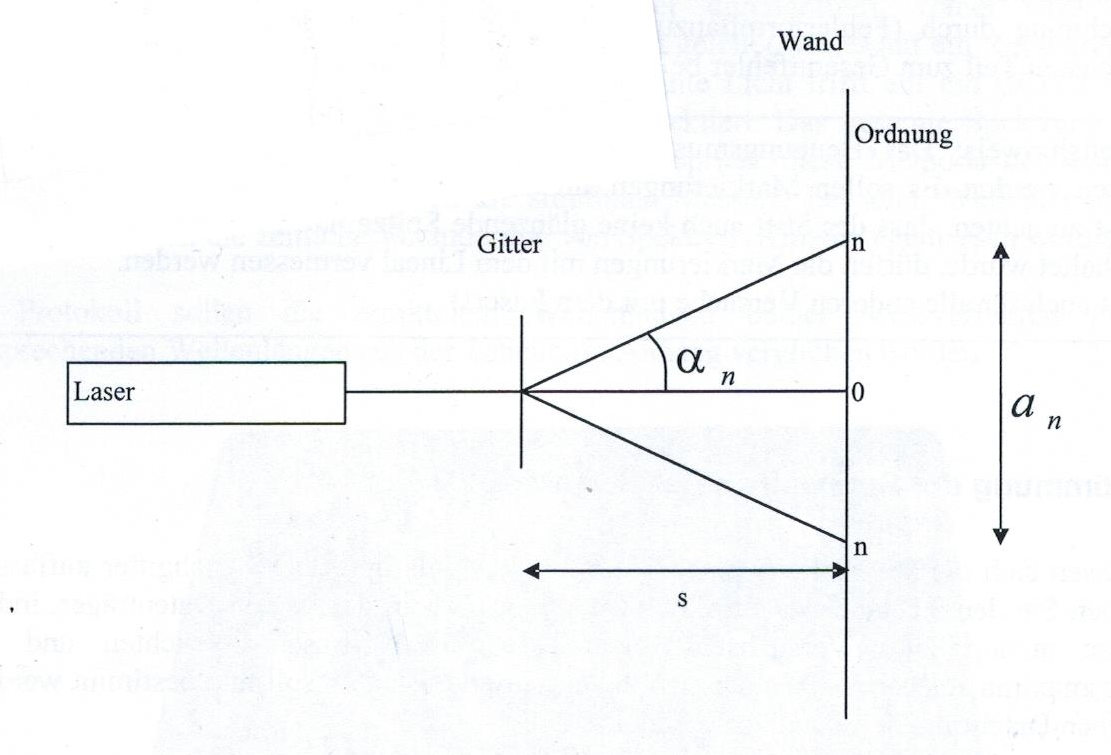
\includegraphics[scale=0.75]{BeugungGitter.PNG}
  \caption{Versuchsaufbau zur Bestimmung der Gitterkonstante (aus der Versuchsanleitung)}
  \label{fig:Gitter}
\end{figure}
Für jedes Maximapaar der Ordnung $n$ wird bis $n = 3$ jeweils der Abstand $a_{n}$ zwischen den beiden Maxima gemessen. Mit dem Winkel $\alpha_{n}$ zwischen dem Laserstrahl und der Strecke Gitter-Maximum kann dann die Gitterkonstante berechnet werden:
\begin{align}
g = \dfrac{n \lambda}{sin \left( \alpha_{n} \right) }
\end{align}
$\alpha_{n}$ wird mit dem konstanten Abstand $s$ zwischen Gitter und Wand bestimmt durch $tan (\alpha_{n}) = \dfrac{a_{n}}{2s}$, deshalb ergibt sich für $g$:
\begin{align}
g = \dfrac{n \lambda}{sin \left( arctan \left( \dfrac{a_{n}}{2s} \right) \right) }
\label{eq:Gitter1}
\end{align}
In diesem Versuch ist $\alpha_{n}$ klein, deshalb wird die Kleinwinkelnäherung $tan (\alpha_{n}) \cong sin (\alpha_{n})$ verwendet:
\begin{align}
g \cong \dfrac{n \lambda}{tan \left( arctan \left( \dfrac{a_{n}}{2s} \right) \right) } = \dfrac{2n \lambda s}{a_{n}}
\label{eq:Gitter2}
\end{align}

\subsection{Fehlerrechnung}
Der Größtfehler $\Delta g$ der Gitterkonstante mit Gleichung \ref{eq:Gitter2} beträgt
\begin{align*}
\Delta g & = \left| \dfrac{\partial g}{\partial s} \right| \Delta s + \left| \dfrac{\partial g}{\partial a_{n}} \right| \Delta a_{n} = \left| \dfrac{2n \lambda}{a_{n}} \right| \Delta s + \left| 2n \lambda s \cdot \dfrac{-1}{a_{n}^{2}} \right| \Delta a_{n} = \dfrac{2n \lambda}{a_{n}} \cdot \left( \Delta s + \dfrac{s}{a_{n}} \Delta a_{n} \right)
\end{align*}
Mit den Größtfehlern $\Delta s = 0,005m$ und $\Delta a_{n} = 0,002m$ ergeben sich  die Werte aus Tabelle \ref{tab:Gitter} für $\Delta g$.
\subsection{Messwerte und Ergebnisse}
Bekannte Wellenlänge des Lasers: $\lambda = 632,8nm = 6,328 \cdot 10^{-7}m$ \\
Messung des Abstands Gitter-Wand: $s = 1,975m$
Tabelle \ref{tab:Gitter} zeigt für jede Ordnung $n$ die Abstandsmessung $a_{n}$ zwischen den Maxima, das Ergebnis für $g$ und den Größtfehler $\Delta g$.
\begin{table}[H]
\captionof{table}{Maxima-Abstand $a_{n}$, damit errechnete Gitterkonstante $g$ und deren Größtfehler $\Delta g$ nach Ordnungen $n$ der Maxima}
\begin{center}
\begin{tabular}{l|l|l|l}
$n$    & $a_{n}$ {[}m{]} & $g$ {[}m{]} & $\Delta g$ {[}m{]}\\
\hline
1          & 0,248       & $1,008 \cdot 10^{-5}$ & $1,068 \cdot 10^{-7}$ \\
2          & 0,504       & $9,919 \cdot 10^{-6}$ & $6,477 \cdot 10^{-8}$ \\
3          & 0,773       & $9,701 \cdot 10^{-6}$ & $4,966 \cdot 10^{-8}$ \\
\hline
Mittelwert &             & $9,900 \cdot 10^{-6}$ & $7,364 \cdot 10^{-8}$
\end{tabular}
\end{center}
\label{tab:Gitter}
\end{table}

\subsection{Ergebnisdiskussion}
Der tatsächliche Wert für die Gitterkonstante ist mit $10 \mu m = 10^{-5} m$ angegeben. Diesen unterschreitet der Mittelwert um 1\% und liegt damit außerhalb des Größtfehlerintervalls. Diese Abweichung ist akzeptabel, da bei der Bestimmung von $g$ die Kleinwinkelnäherung in Gleichung \ref{eq:Gitter2} statt der genauen Gleichung \ref{eq:Gitter1} genutzt wurde.

\section{Bestimmung der Spurweite einer CD bzw. DVD}
\subsection{Versuchsdurchführung}
Ziel des Versuches ist es, die Spurweite eines Datenträgers zu berechnen und damit zu bestimmen, ob es sich um eine CD oder um eine DVD handelt. Dazu wird dasselbe Vorgehen wie bei der Berechnung der Gitterkonstante im vorherigen Abschnitt angewandt, diesmal ist $g$ die Spurweite. Es wird wieder der HeNe-Laser verwendet, die CD ersetzt das Gitter. Es werden nur die Maxima erster Ordnung betrachtet, da die Maxima höherer Ordnung nicht zu erkennen sind. Der Laser muss dieses Mal etwas näher zur Wand gerückt werden, da die Winkel $\alpha_{n}$ wesentlich größer als beim Gitter sind. Daher wird die Berechnung per Kleinwinkelnäherung (Gleichung \ref{eq:Gitter2}) zu ungenau, stattdessen wird der genaue Wert mit Gleichung \ref{eq:Gitter1} berechnet.
\subsection{Messwerte und Ergebnisse}
Bekannte Wellenlänge des Lasers: $\lambda = 632,8nm = 6,328 \cdot 10^{-7}m$ \\
Messung des Abstands CD-Wand: $s = 0,196m$ \\
Abstand der Maxima: $a_{n} = 0,185m$
\begin{align*}
g = \dfrac{n \lambda}{sin \left( arctan \left( \dfrac{a_{n}}{2s} \right) \right) } = \dfrac{1 \cdot 6,328 \cdot 10^{-7}m}{sin \left( arctan \left( \dfrac{0,185m}{2 \cdot 0,196m} \right) \right) } = 1,483 \cdot 10^{-6}m
\end{align*}
\subsection{Ergebnisdiskussion}
Da der tatsächliche Werte für die Spurweite einer CD mit $1,6 \mu m = 1,6 \cdot 10^{-6}m$, einer DVD mit $0,74 \mu m$ und einer Blu-ray mit $0,32 \mu m$ in der Versuchsanleitung angegeben ist, muss es sich bei dem Datenträger um eine CD handeln. Die berechnete Spurweite unterschreitet die tatsächliche also um 7,3\%. Gründe für diese Abweichung sind wohl Fehler bei der Messung von $a_{n}$ und $s$, sowie eine nicht genau senkrechte Ausrichtung des Lasers zur Wand.

\section{Spektralanalyse (Untersuchung einer unbekannten Lichtquelle)}
\subsection{Versuchsdurchführung}
\subsection{Messwerte und Ergebnisse}
\subsection{Ergebnisdiskussion}

\section{Strukturaufklärung (Bestimmung einer Gitterkonstanten)}
\subsection{Versuchsdurchführung}
\subsection{Messwerte und Ergebnisse}
\subsection{Ergebnisdiskussion}

\section{Strukturaufklärung (Bestimmung einer Gitterkonstanten)}
\subsection{Versuchsdurchführung}
\subsection{Messwerte und Ergebnisse}
\subsection{Ergebnisdiskussion}
Bei kleiner werdender Spaltbreite werden die Maxima breiter und auseinandergezogen.
\end{document}